\subsection{RailTopoModel}

    En 2016 la UIC (del inglés, International Union of Railways) publicó el Standard 30100 \cite{Paper_109} en el cual definió un formato de intercambio de datos ferroviarios llamado RailTopoModel \cite{Paper_146,Paper_149,Paper_150,Paper_200}. RailTopoModel es un modelo topológico de infraestructura ferroviaria basado en grafos. El modelo abarca tres tipos de niveles, la topología de la red, objetos materiales, objetos inmateriales y objetos lógicos \cite{Paper_109}, tal como se ilustra en la Figura \ref{fig:RTM_3} (adaptada al español de \cite{Paper_109}). 

    \begin{figure}[H]
        \centering
        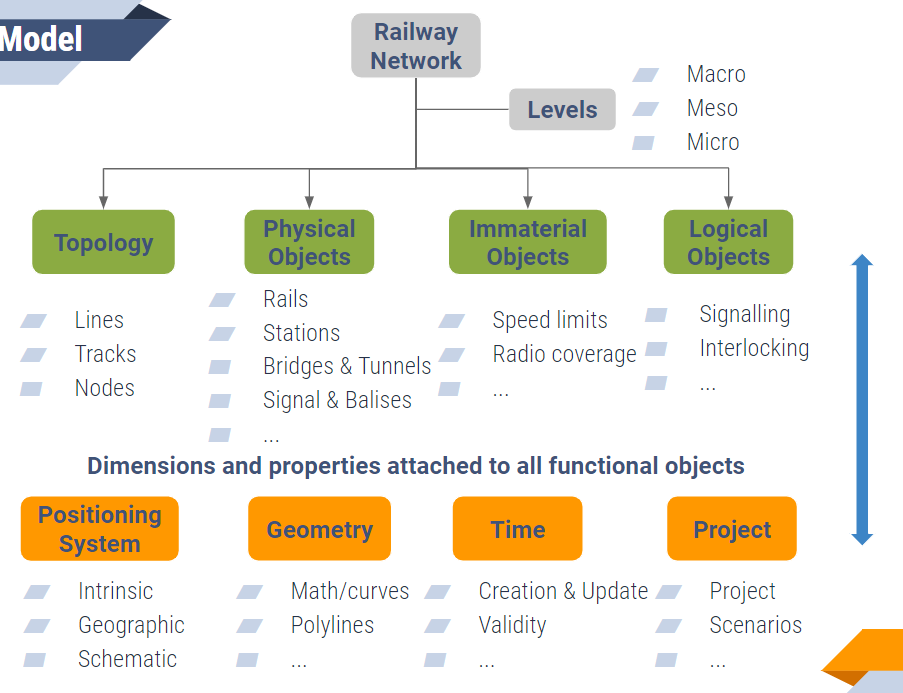
\includegraphics[width=1\textwidth]{Figuras/objetos}
        \centering\caption{Alcance del modelo de UIC RailTopoModel.}
        \label{fig:RTM_3}
    \end{figure}

    Cada uno de estos elementos posee propiedades y características propias, que pueden ser físicas o abstractas. Por ejemplo, los objetos materiales pueden ser adimensionales (señales, balizas, etc), unidimensionales (vías, plataformas, etc) o bidimensionales (estaciones, túneles, etc). Debido a como fue diseñado, RailTopoModel es el modelo ideal para implementar un enfoque geográfico \cite{Paper_146,Paper_149,Paper_180,Paper_182,Paper_99,Paper_107}.
    
\subsubsection{Paquete base}

    El estándar RailTopoModel se divide en cuatro paquetes: la base, la topología, el posicionamiento y la red de entidades. La base incluye toda la información de alto nivel de la infraestructura que son comúnes a toda la red \cite{Paper_146}. Por ejemplo, el sistema de alimentación eléctrico utilizado puede ser por tercer riel o catenarias y este no cambia a lo largo de toda la red.

\subsubsection{Modelo de grafos}
    \label{sec:RTM}
    
    En el pasado, otros estudios han tratado de modelar el trazado ferroviario utilizando teoría de grafos \cite{Paper_9,Paper_101,Paper_102,Paper_103}. Pero todos ellos definían a las vías como las aristas del grafo y los cambios de vías como los nodos, lo cual dificultaba enormemente la inclusión de otros elementos ferroviarios como las plataformas, los pasos a nivel o los semáforos. RailTopoModel se apega mas a la teoría clásica de grafos y define como nodos a la unidad mínima de recursos físicos, llamándolos netElements y a la conexión física entre ellos como aristas, llamándolos netRelations \cite{Paper_109}.

    Un netElement debe contener un tramo de vía en su totalidad o varios tramos, pero un tramo de vía no puede tener varios netElements asociados. Opcionalmente, un netElement puede tener además cualquier otro elemento ferroviario asociado como plataformas, semáforos o balizas. Para entender mejor como se materializa este concepto se tiene la Figura \ref{fig:grafos_1} (adaptada al español de \cite{Paper_109}) que ejemplifica el modelado en grafos de una maquina de cambios.

    \begin{figure}[H]
        \centering
        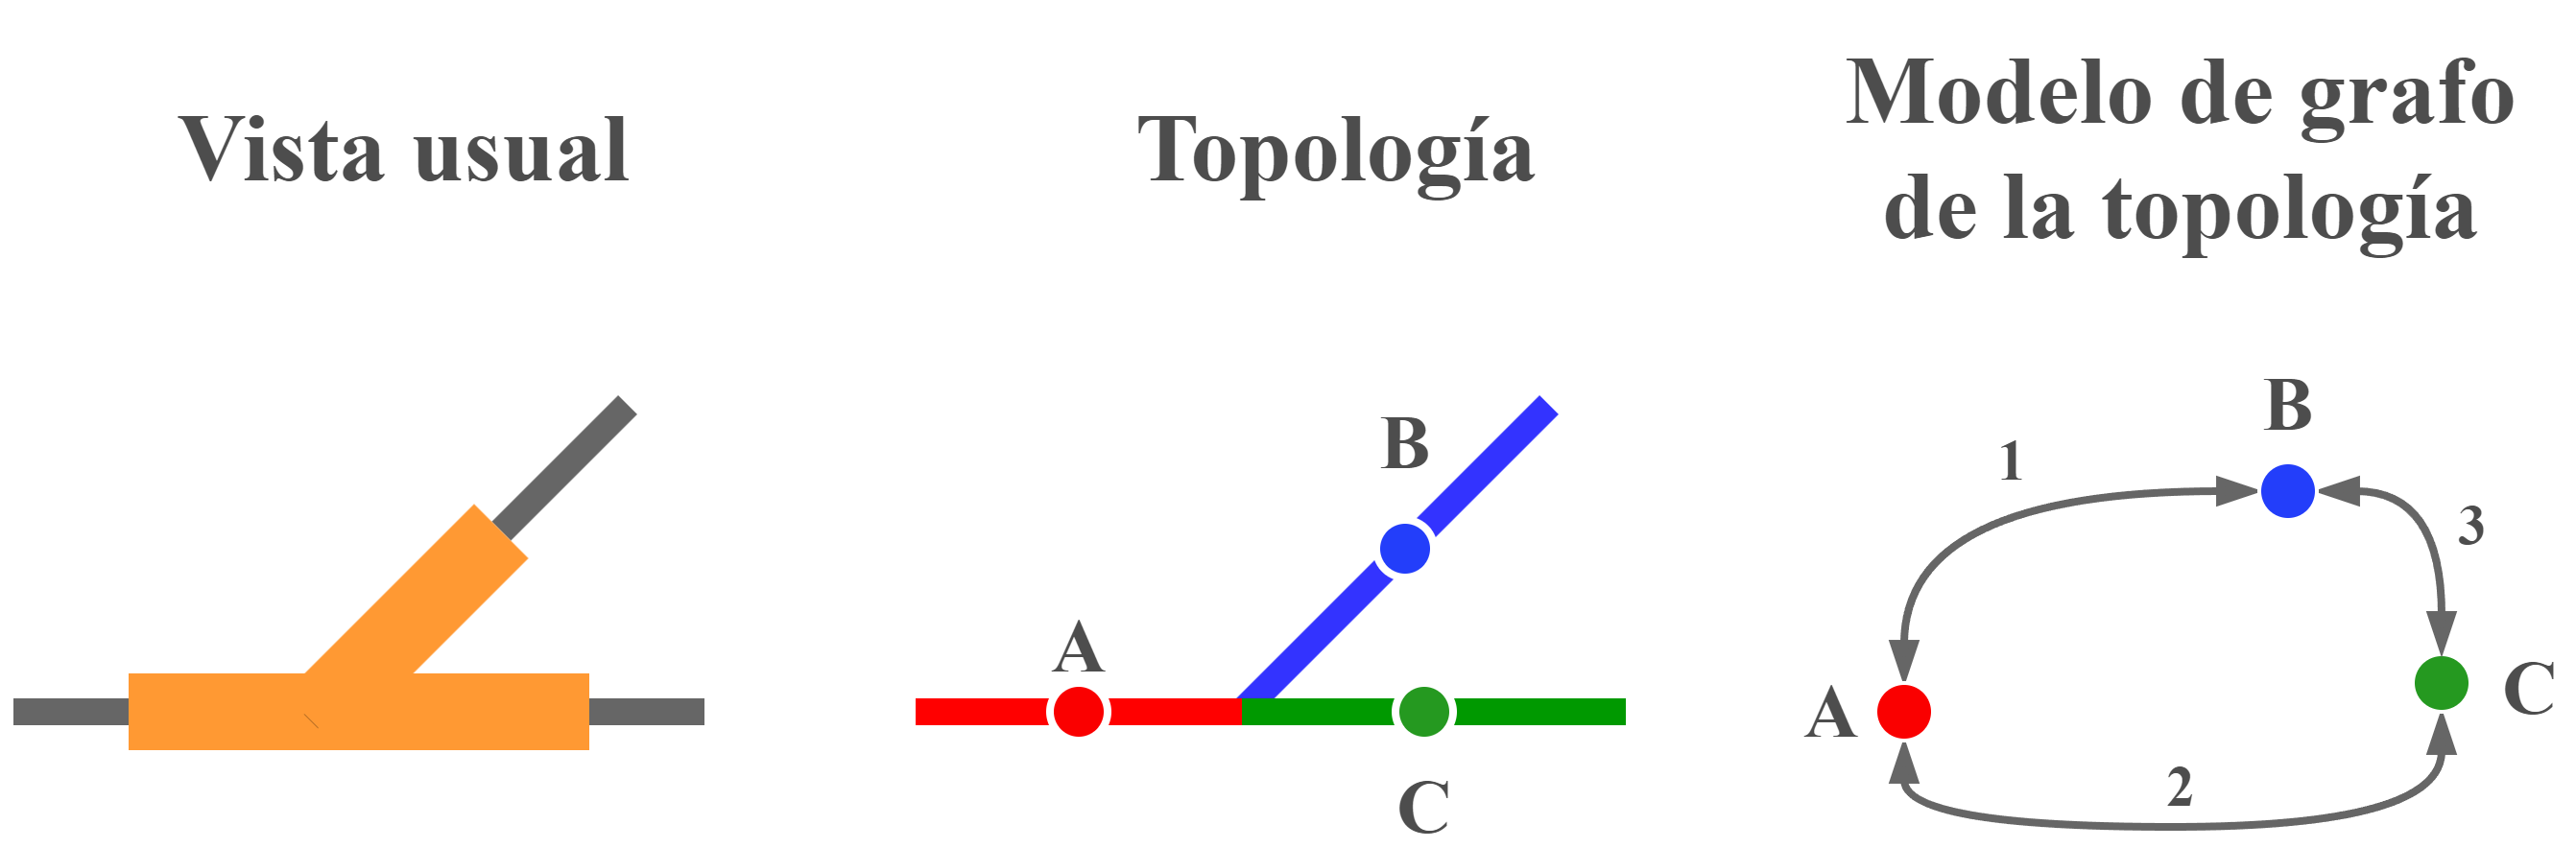
\includegraphics[width=1\textwidth]{Figuras/grafos}
        \centering\caption{Modelado en grafos de un cambio de vías simple.}
        \label{fig:grafos_1}
    \end{figure}

    En la Figura \ref{fig:grafos_1} se tiene un cambio de vías simple que conecta una vía de circulación (horizontal) con una vía de maniobras (oblicua). El netElement asociado a la vía principal antes de la bifurcación lo llamaremos A. Este netElement es también al que se asocia al objeto del cambio de vías simple. El netElement asociado a la vía de maniobras lo denominamos B y al asociado a la vía de continuación de la circulación lo denominamos C.

    En la representación del modelo de grafos, el netRelation 1 relaciona el netElement A y B de forma biyectiva. Es decir, A esta relacionado con B y B está relacionado con A. De la misma forma se asignan los netRelations 2 y 3. Sin embargo, no hay que confundir que dos vías estén conectadas con que un tren puede circular por ellas. Una formación podría circular por el tramo A-C, A-B, B-A y C-A, pero no podrá circular desde B hacia C sin pasar por A o viceversa. Es físicamente imposible que un tren realice ese movimiento de una sola maniobra. Para circular desde B hacia C primero deberá finalizar el tramo B-A, modificar la posición de la máquina de cambios y recorrer el tramo A-C. A la propiedad asignada a los netRelation que son físicamente transitables se la denomina navegabilidad y es una característica esencial de las redes de grafos que modelan redes ferroviarias. En este ejemplo, solo los netRelation 1 y 2 poseen navegabilidad. Los cambios de vías, sean estos simples, dobles o en tijeras, son los únicos elementos ferroviarios que alteran de forma dinámica la red ferroviaria y, por lo tanto, los únicos que afectan al parámetro de navegabilidad en los netElements adyacentes.
    
    
\subsubsection{Topología y niveles}

    La topología del modelo es una parte fundamental del estándar. RailTopoModel incluye el "principio de agregación", por el cual los elementos pueden ser agrupados en entidades mas grandes. En la Figura \ref{fig:RTM_1} se puede visualizar la estructura de capas propuesto por RailTopoModel (adaptada al español de \cite{Paper_109}).

    \begin{figure}[H]
        \centering
        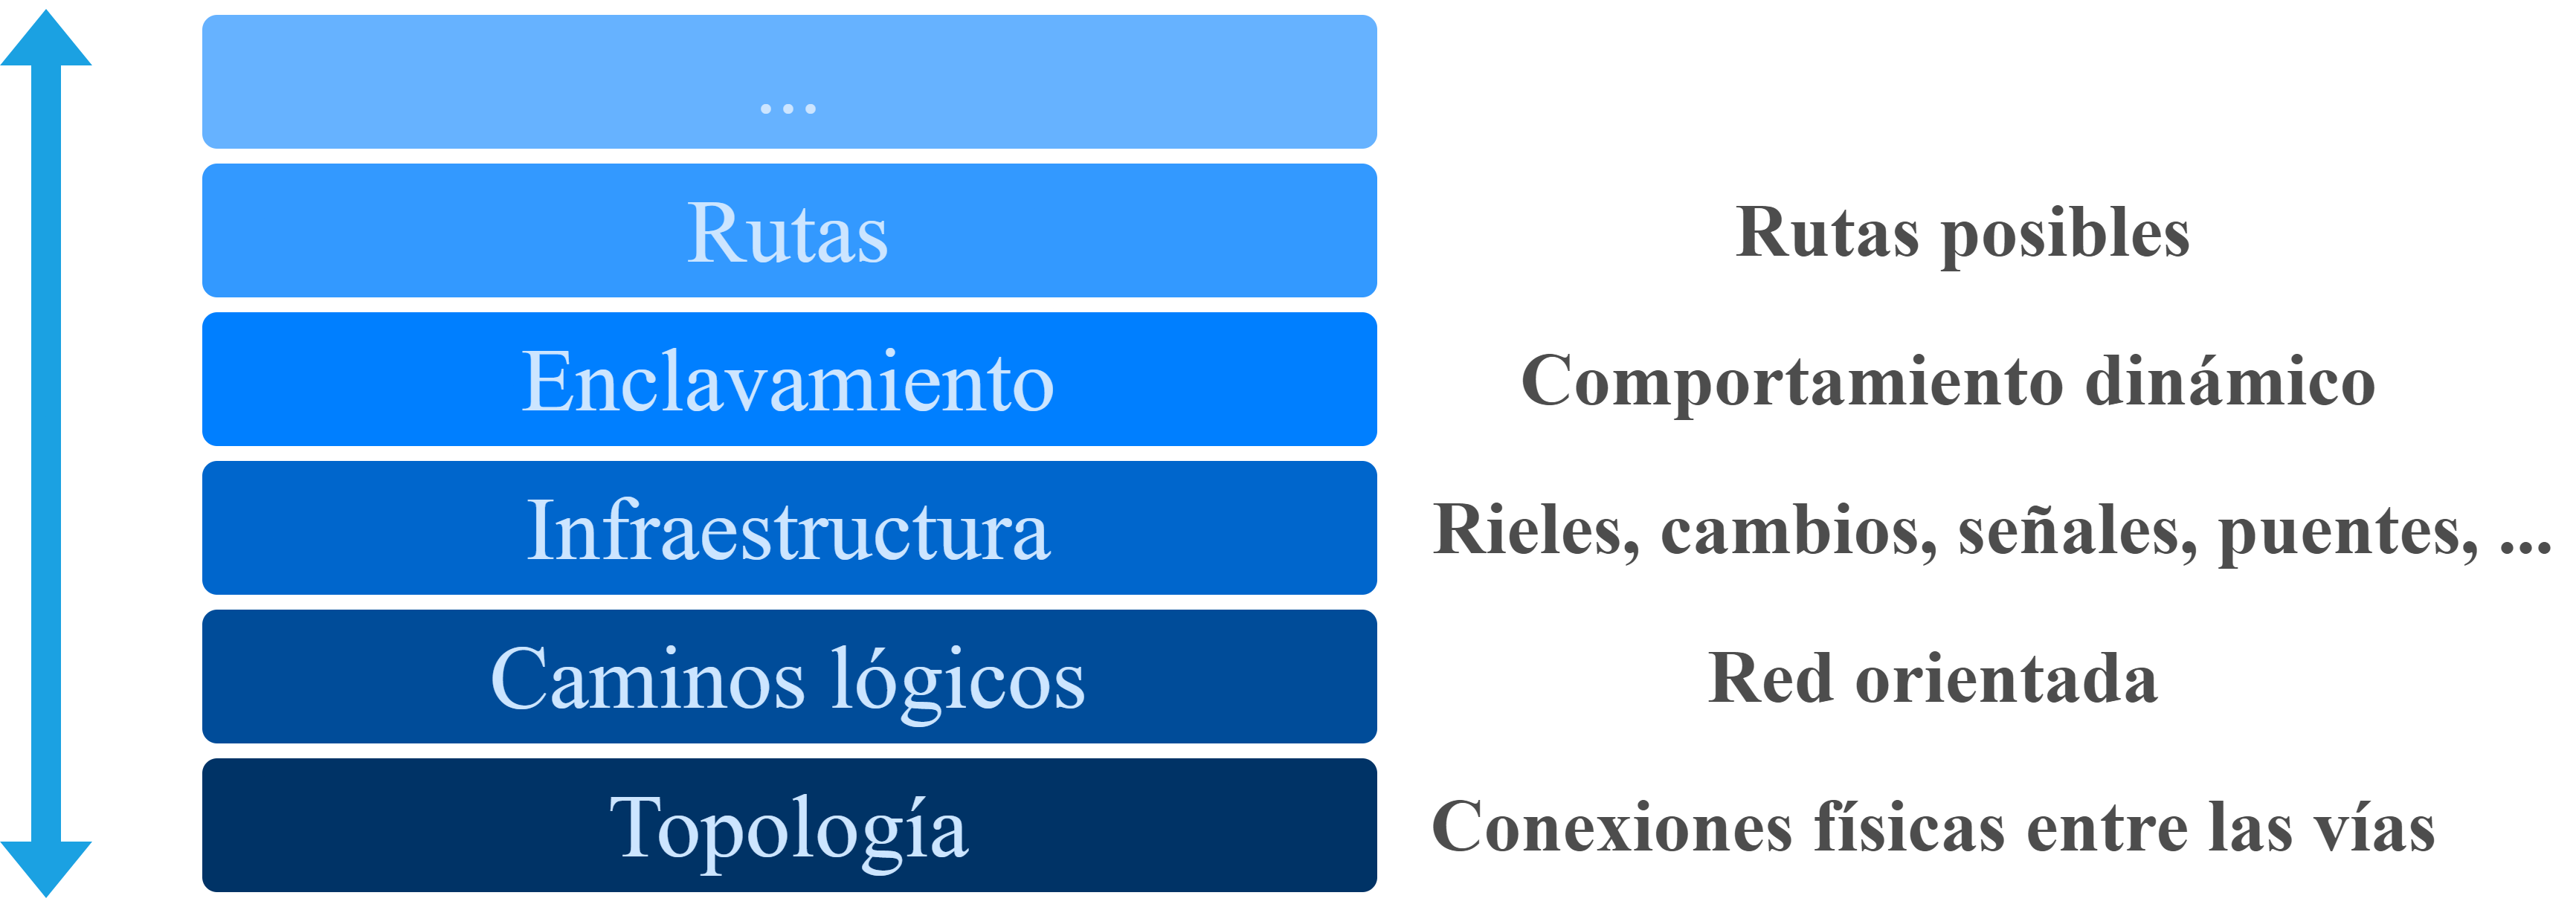
\includegraphics[width=1\textwidth]{Figuras/capas}
        \centering\caption{Estructura de capas de RailTopoModel.}
        \label{fig:RTM_1}
    \end{figure}
    
    La topología de la red está compuesta por los nodos (netElements) y las aristas (netRelations) que los conectan entre sí, lo cual constituye el nivel microscópico de la red. Cada nodo representa un tramo de vías que puede tener ciertos elementos ferroviarios asociados o ninguno. A su vez, los nodos pueden ser agrupados en diversos caminos lógicos, que son el conjunto de nodos cuyas relaciones y navegabilidad les permite constituir un camino físico entre ellos \cite{Paper_150}.

    A medida que se agrupan mas y mas cambios de vías junto con las plataformas y máquinas de cambios se constituye un punto de operación. La descripción en base a puntos de operación es a nivel mesoscópico, como se muestra en la Figura \ref{fig:RTM_2} (adaptada al español de \cite{Paper_109}), y es utilizado en logística. Las secciones de vía que no incluyen plataformas en las cuales las formaciones puedan detenerse se denominan secciones de líneas, o simplemente "líneas" dentro del modelo de RailTopoModel. La descripción que incluye tanto los puntos de operación como las secciones de líneas es a nivel macroscópico \cite{Paper_149}. Esta simplificación de la red es de gran importancia, ya que es ampliamente utilizada en los mapas ferroviarios de todas las estaciones del mundo: los puntos de operación son las estaciones y las secciones de línea son las vías que las comunican. 
    
    \begin{figure}[H]
        \centering
        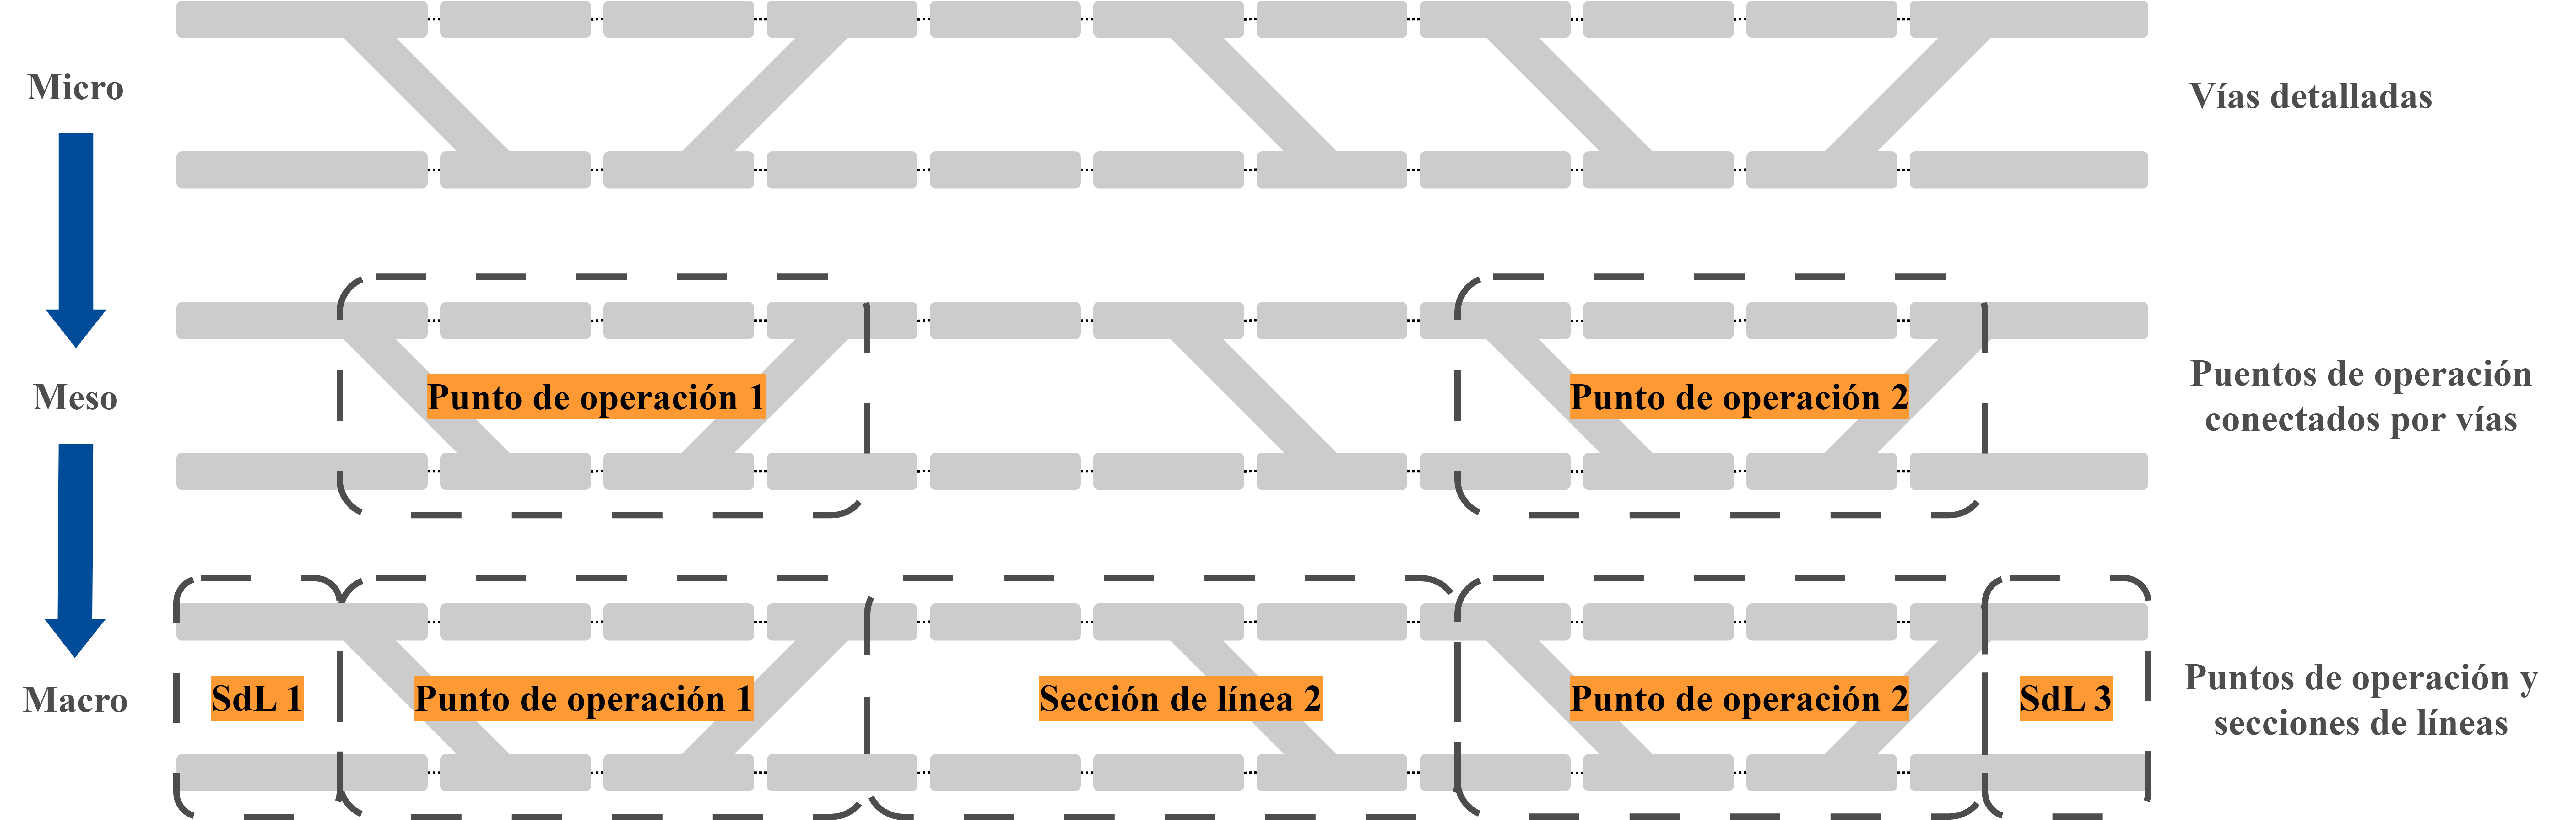
\includegraphics[width=1\textwidth]{Figuras/railtopomodel}
        \centering\caption{Niveles microscópico, mesoscópico y macroscópico.}
        \label{fig:RTM_2}
    \end{figure}
    
    Las instalaciones y sus propiedades constituyen todos los elementos ferroviarios asociados a un nodo. Estos representan elementos físicos del mundo real, pueden ser estáticos o dinámicos. Los elementos estáticos como los puentes, curvas y estaciones no alteran sus propiedades en ningún momento. Los elementos dinámicos como los pasos a nivel, máquinas de cambios o señales tienen algunas propiedades fijas, como la posición física del elemento, pero otras variables, como la posición mecánica de alguna de sus piezas o el estado eléctrico de sus circuitos \cite{Paper_146,Paper_150}.

    Un sistema de enclavamiento relaciona todos los módulos previamente mencionados. El sistema de enclavamientos modificará el estado de los elementos dinámicos, basados en el estado actual de los mismos, sometido a las restricciones impuestas por los elementos estáticos, buscando habilitar los caminos lógicos mas cortos y seguros entre un punto A y B.

    Finalmente, las rutas permitidas se obtienen a partir del estado de los elementos dinámicos decidido por el sistema y de definir el camino óptimo entre A y B que no comprometa la infraestructura del sistema. Todas las restricciones impuestas por las capas inferiores (caminos lógicos posibles, limitaciones de la infraestructura o estados previos que sean incompatibles con lo pedido) terminan emergiendo como un conjunto de rutas posibles de ser utilizadas, en detrimento de otras que, en ese instante de tiempo, no podrán ser habilitadas hasta que el estado del sistema se modifique.

    Como se puede apreciar, en este modelo, las rutas son una consecuencia de la infraestructura que se tiene y de los estados anteriores del sistema, producto de las rutas previamente pedidas. Un análisis completo de la topología e infraestructura permitiría obtener todo el conjunto de rutas posibles, para cualquier estado alcanzable por el sistema \cite{Paper_150}.
\subsubsection{Posicionamiento}

    RailTopoModel utiliza diferentes sistemas de posicionamiento: intrínseco, geográfico y esquemático \cite{Paper_112,Paper_150}. Las coordenadas intrínsecas se encuentran en el rango 0 a 1, relativas a la posición dentro del netElement. Estas coordenadas son obligatorias, junto con el largo asociado al netElement, independientemente de si se definieron o no las demás coordenadas. Las coordenadas geográficas son coordenadas absolutas, por ejemplo de un sistemas GPS. Finalmente las coordenadas esquemáticas son relativas a la posición del elemento dentro del archivo que modele ese sistema, muchas veces utilizadas en herramientas de software para posicionar los elementos en una interfaz gráfica.

